%--------------------------------------------------
% Resume in Latex 
% Test Run Commit Line for trigger action
% Author Sagar Parmar
% License : MIT
%--------------------------------------------------

%---- Start of Required Packages and Functions ----

\documentclass[a4paper,11pt]{article}

\usepackage{latexsym}
\usepackage{xcolor}
\usepackage{float}
\usepackage{ragged2e}
\usepackage[empty]{fullpage}
\usepackage{wrapfig}
\usepackage{lipsum}
\usepackage{tabularx}
\usepackage{titlesec}
\usepackage{geometry}
\usepackage{marvosym}
\usepackage{verbatim}
\usepackage{enumitem}
\usepackage[hidelinks]{hyperref}
\usepackage{fancyhdr}
\usepackage{fontawesome5}
\usepackage{multicol}
\usepackage{multirow}
\usepackage{graphicx}
\usepackage{cfr-lm}
\usepackage[T1]{fontenc}
\usepackage[most]{tcolorbox}
\usepackage{ragged2e}

\setlength{\multicolsep}{0pt} 
\pagestyle{fancy}
\fancyhf{} % clear all header and footer fields
\setlength{\footskip}{4.08003pt} %Added new line
\fancyfoot{}
\renewcommand{\headrulewidth}{0pt}
\renewcommand{\footrulewidth}{0pt}
\geometry{left=1.4cm, top=0.8cm, right=1.2cm, bottom=1cm}
\graphicspath{ {./} }

% Adjust margins
%\addtolength{\oddsidemargin}{-0.5in}
%\addtolength{\evensidemargin}{-0.5in}
%\addtolength{\textwidth}{1in}

\tcbset{
  frame code={}
  center title,
  left=0pt,
  right=0pt,
  top=0pt,
  bottom=0pt,
  colback=gray!20,
  colframe=white,
  width=\dimexpr\textwidth\relax,
  enlarge left by=-2mm,
  boxsep=4pt,
  arc=0pt,outer arc=0pt,
}

\urlstyle{same}
\raggedright
\setlength{\tabcolsep}{0in}

% Sections formatting
\titleformat{\section}{
  \vspace{-4pt}\scshape\raggedright\large
}{}{0em}{}[\color{black}\titlerule \vspace{-7pt}]

%--------------------------------------------------

% Custom commands
\newcommand{\resumeItem}[2]{
  \item{
    \textbf{#1}{\hspace{0.5mm}#2 \vspace{-0.5mm}}
  }
}

\newcommand{\resumePOR}[3]{
\vspace{0.5mm}\item
    \begin{tabular*}{0.97\textwidth}[t]{l@{\extracolsep{\fill}}r}
        \textbf{#1}\hspace{0.3mm}#2 & \textit{\small{#3}} 
    \end{tabular*}
    \vspace{-2mm}
}

\newcommand{\resumeSubheading}[4]{
\vspace{0.5mm}\item
    \begin{tabular*}{0.98\textwidth}[t]{l@{\extracolsep{\fill}}r}
        \textbf{#1} & \textit{\footnotesize{#4}} \\
        \textit{\footnotesize{#3}} &  \footnotesize{#2}\\
    \end{tabular*}
    \vspace{-2.4mm}
}

\newcommand{\resumeProject}[4]{
\vspace{0.5mm}\item
    \begin{tabular*}{0.98\textwidth}[t]{l@{\extracolsep{\fill}}r}
        \textbf{#1} & \textit{\footnotesize{#3}} \\
        \footnotesize{\textit{#2}} & \footnotesize{#4}
    \end{tabular*}
    \vspace{-2.4mm}
}

\newcommand{\resumeSubItem}[2]{\resumeItem{#1}{#2}\vspace{-4pt}}

% Bullet Section Starts
% \renewcommand{\labelitemii}{$\circ$}
\renewcommand{\labelitemi}{} %No bullets
%\renewcommand{\labelitemi}{$\vcenter{\hbox{\tiny$\bullet$}}$} %Add bullets
% Bullet Section Ends

\newcommand{\resumeSubHeadingListStart}{\begin{itemize}[leftmargin=*,labelsep=0mm]}
\newcommand{\resumeHeadingSkillStart}{\begin{itemize}[leftmargin=*,itemsep=1.7mm, rightmargin=2ex]}
\newcommand{\resumeItemListStart}{\begin{justify}\begin{itemize}[leftmargin=3ex, rightmargin=2ex, noitemsep,labelsep=1.2mm,itemsep=0mm]\small}
\newcommand{\resumeSubHeadingListEnd}{\end{itemize}\vspace{2mm}}
\newcommand{\resumeHeadingSkillEnd}{\end{itemize}\vspace{-2mm}}
\newcommand{\resumeItemListEnd}{\end{itemize}\end{justify}\vspace{-2mm}}
\newcommand{\cvsection}[1]{%
\vspace{2mm}
\begin{tcolorbox}
    \textbf{\large #1}
\end{tcolorbox}
    \vspace{-4mm}
}
\newcolumntype{L}{>{\raggedright\arraybackslash}X}%
\newcolumntype{R}{>{\raggedleft\arraybackslash}X}%
\newcolumntype{C}{>{\centering\arraybackslash}X}%
%---- End of Packages and Functions ------

%--------------------------------------------------

% ==================== CV STARTS HERE  ====================

%%%%%% DEFINE ELEMENTS STARTS HERE %%%%%%%
\newcommand{\name}{Sagar Parmar Test} % Your Name
\newcommand{\role}{Software Engineer} % Your Name
\newcommand{\course}{Computer Science and Engineering} % Your Program
\newcommand{\phone}{97144 66108} % Your Phone Number
\newcommand{\emaila}{sagarparmar881@gmail.com} %Email Address
\newcommand{\home}{Vadodara, Gujarat} %Home
\newcommand{\website}{sagarparmar881.github.io} %Website
\newcommand{\about}{I am Sagar, a software engineer proficient in Python, Java, C/C++ and a few more. Experienced in web development with frameworks like React, Vue and Spring. I am well-versed in DevOps tools like Jenkins, Docker and Maven. With a strong understanding of databases such as MySQL and MongoDB, I excel in building robust applications. My passion for continuous learning and adapting to new technologies drives my commitment to delivering innovative solutions.} %About You
%%%%%% DEFINE ELEMENTS ENDS HERE %%%%%%%

\begin{document}

\fontfamily{cmr}\selectfont
%----------HEADING-----------------

{ \renewcommand{\arraystretch}{1.15}



%+-+-+-+-+-+-+-+-+-+-+-+-+-+-+-+-+-+-+-+-+-+-+-+-+-+-+-+-+-+-+
% ---- DETAILS SECTION STARTS ----
%+-+-+-+-+-+-+-+-+-+-+-+-+-+-+-+-+-+-+-+-+-+-+-+-+-+-+-+-+-+-+

% This section is displayed in two-columned table. 
% [Col01-Details & Col02-ProfilePicture] 

\begin{tabularx}{\linewidth}{L r} \textbf{\LARGE \name}
\vspace{2mm} 
& \multirow{6}{*}{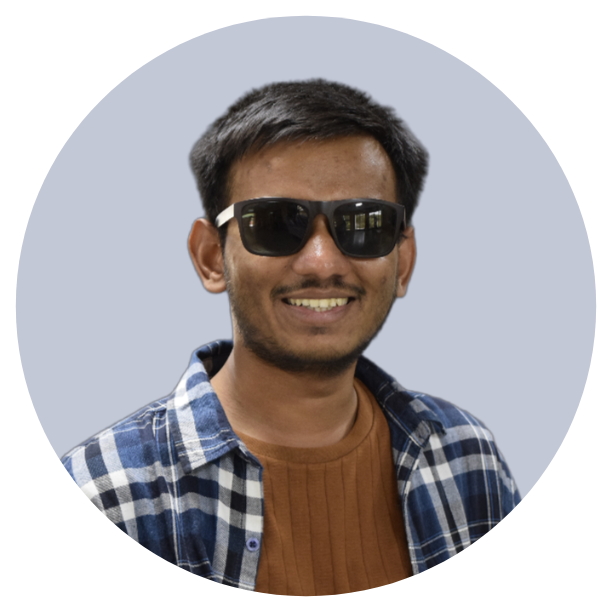
\includegraphics[height=3cm]{sagar}} \\ % [Col1-Space & Col02-Image(x/6Col)]

\textbf{\normalsize \role} & \\
{\raisebox{0.0\height}{\footnotesize \faPhone}\ +91-\phone} & \\ % [Col1-Phone & Col02-Image(x/6Col)]

\href{mailto:\emaila}{\raisebox{0.0\height}{\footnotesize
\faEnvelope}\ {\emaila}} & \\ % [Col1-Email & Col02-Image(x/6Col)]


\href{https://github.com/sagarparmar881}{\raisebox{0.0\height}{\footnotesize
\faGithub}\ {sagarparmar881}} & \\ % [Col1-Github & Col02-Image(x/6Col)]

{\raisebox{0.0\height}{\footnotesize \faHome}\ \home} & \\ % [Col1-Home & Col02-Image(x/6Col)]

\href{https://sagarparmar881.github.io/}{\raisebox{0.0\height}{\footnotesize
\faGlobe}\ \website} & \\ \end{tabularx}  % [Col1-Website & Col02-Image(x/6Col)]

}
% ---- DETAILS SECTION ENDS ----


%+-+-+-+-+-+-+-+-+-+-+-+-+-+-+-+-+-+-+-+-+-+-+-+-+-+-+-+-+-+-+
% ---- ABOUT ME SECTION STARTS ----
%+-+-+-+-+-+-+-+-+-+-+-+-+-+-+-+-+-+-+-+-+-+-+-+-+-+-+-+-+-+-+
\section{\textbf{About Me}}
\justifying
\about
\vspace{-1.5mm}
% ---- ABOUT ME SECTION ENDS ----


%+-+-+-+-+-+-+-+-+-+-+-+-+-+-+-+-+-+-+-+-+-+-+-+-+-+-+-+-+-+-+
% ---- EDUCATION SECTION STARTS ----
%+-+-+-+-+-+-+-+-+-+-+-+-+-+-+-+-+-+-+-+-+-+-+-+-+-+-+-+-+-+-+
\section{\textbf{Education}}
\resumeSubHeadingListStart

\resumeSubheading
{Navrachana University, Vadodara}{CGPA: 8.62}
{Masters of Technology in Computer Science and Engineering}{2021-23}

\resumeSubheading
{Navrachana University, Vadodara}{CGPA: 8.17}
{Bachelors of Technology in Computer Science and Engineering}{2017-21}

\resumeSubheading
{Vidhyut Board Vidhyalaya, Vadodara}{Grade: C1}
{Higher Secondary School Certificate (HSC), Science (PCM)}{March, 2017}

\resumeSubheading
{Kelavani English Medium School, Vadodara}{Grade: B1}
{Secondary School Certificate (SSC)}{March, 2015}

\resumeSubHeadingListEnd
\vspace{-5.5mm}

% ---- EDUCATION SECTION ENDS ----

%+-+-+-+-+-+-+-+-+-+-+-+-+-+-+-+-+-+-+-+-+-+-+-+-+-+-+-+-+-+-+
% ---- PROJECTS SECTION STARTS ----
%+-+-+-+-+-+-+-+-+-+-+-+-+-+-+-+-+-+-+-+-+-+-+-+-+-+-+-+-+-+-+

\section{\textbf{Projects}}
\resumeSubHeadingListStart
%Project[01]
\resumeProject
{Real-Time Face Recognition from Multiple Camera} %Project Name
{This project is to develop a system that can recognize faces from multiple cameras in real-time.} %Project Name, Location Name
{\href{https://github.com/sagarparmar881/real-time-face-recognition-from-multiple-camera}{\raisebox{0.0\height}{\footnotesize \faGithub}\ {View Project}}} %Project Dates/ Link

\resumeItemListStart
\item {Recognition model: Dlib-based ResNet pre-trained model.}
\item {Recognition algorithm : ResNet Neural Network.}
\item {Technology Used: Python3}
\resumeItemListEnd
\vspace{-2mm}

%Project[02]
\resumeProject
{Real-Time Indian License Plate Recognition with Jetson Nano} %Project Name
{This project is implemented on Jetson Nano and its results reached 40 FPS.} %Project Name, Location Name
{\href{https://github.com/sagarparmar881/real-time-indian-license-plate-recognition-with-jetson-nano}{\raisebox{0.0\height}{\footnotesize \faGithub}\ {View Project}}} %Project Dates/ Link

\resumeItemListStart
\item {Model - License Plate Detection: SSD-Mobilenet-v1}
\item {Model - License Plate Recognition: SSD-Mobilenet-v1}
\item {Technology Used: Python3 }
\resumeItemListEnd
\vspace{-2mm}

%Project[03]
\resumeProject
{Navrachana University Website} %Project Name
{Developed "Official University Website" and worked with several technologies}
{\href{https://dkots111.github.io/nuv-website/}{\raisebox{0.0\height}{\footnotesize \faGithub}\
{View Project}}} %Project Dates/ Link

\resumeItemListStart
\item {Technology Used : HTML, CSS, JavaScript, Bootstrap, JQuery and Adobe XD}
\resumeItemListEnd
\resumeSubHeadingListEnd
\vspace{-8.5mm}
% ---- PROJECTS SECTION ENDS ----

%+-+-+-+-+-+-+-+-+-+-+-+-+-+-+-+-+-+-+-+-+-+-+-+-+-+-+-+-+-+-+
% ---- EXPERIENCE SECTION STARTS ----
%+-+-+-+-+-+-+-+-+-+-+-+-+-+-+-+-+-+-+-+-+-+-+-+-+-+-+-+-+-+-+
\section{\textbf{Experience}}
\resumeSubHeadingListStart

%Experience[01]
\resumeSubheading
{Software Engineer}{In-Office}
{NetWeb Software, Vadodara}{Jul, 23 - Present}
\vspace{-2.0mm}
\resumeItemListStart
\item {Developed and maintained software applications using Java, Spring Boot, Scala, React.js, Git, Agile Application Development, REST APIs, and Tortoise SVN.}
\resumeItemListEnd
\vspace{-3.0mm}

%Experience[02]
\resumeSubheading
{Internship Trainee}{In-Office}
{NetWeb Software, Vadodara}{Aug, 22 - Jul, 23}
\vspace{-2.0mm}
\resumeItemListStart
\item {Learned the fundamentals of Spring Boot}
\item {Learned basics of JUnit}
\resumeItemListEnd
\vspace{-3.0mm}

\resumeSubHeadingListEnd
\vspace{-5.5mm}
% ---- EXPERIENCE SECTION ENDS ----


%+-+-+-+-+-+-+-+-+-+-+-+-+-+-+-+-+-+-+-+-+-+-+-+-+-+-+-+-+-+-+
% ---- TECHNICAL SKILLS SECTION STARTS ----
%+-+-+-+-+-+-+-+-+-+-+-+-+-+-+-+-+-+-+-+-+-+-+-+-+-+-+-+-+-+-+
\section{\textbf{Technical Skills and Interests}}
\vspace{2mm}
\begin{itemize}[leftmargin=0.05in, label={}]
  \small{\item{
        \textbf{Platforms}{: Windows, Linux, Mac } \\
        \textbf{Programming Languages}{: C, C++, Python, Java, Scala, SQL, Dart, HTML+CSS } \\
        \textbf{Scripting Languages}{: Javascript, PHP, R, Bash, VBA }\\
        \textbf{Frameworks}{: Express, Django, Laravel, Spring, Angular, React, Vue } \\
        \textbf{Database}{: Oracle, MySQL, MongoDB } \\
        \textbf{DevOps}{: Git, Maven, Jenkins, Docker, Selenium, Gradle } \\
        \textbf{Web Services}{: RESTful APIs } \\
        \textbf{Web Servers}{: Apache HTTP Server, Apache Tomcat, NGINX, NodeJS } \\
        \textbf{Cloud Computing}{: DigitalOcean, Linode, AWS, Azure, Hostinger} \\
        \textbf{Cloud Platforms}{: Jira, Confluence, Vercel} \\
        \textbf{Tools}{: JMeter, Visual Studio, Eclipse} \\

        }}
\end{itemize}
\vspace{-12pt}
% ---- TECHNICAL SKILLS SECTION ENDS ----

%+-+-+-+-+-+-+-+-+-+-+-+-+-+-+-+-+-+-+-+-+-+-+-+-+-+-+-+-+-+-+
% ---- CERTIFICATIONS SECTION STARTS ----
%+-+-+-+-+-+-+-+-+-+-+-+-+-+-+-+-+-+-+-+-+-+-+-+-+-+-+-+-+-+-+
\section{\textbf{Certifications}}
\resumeSubHeadingListStart

\resumeProject
{Jetson AI Specialist Certificate (2022)} %Project Name
{NVIDIA Jetson} %Credential ID/ Year
{\href{https://drive.google.com/file/d/1q0Z_5TkDHRhdkgCClicprZhJg2su5BDk/view}{\raisebox{0.0\height}{\footnotesize \faGithub}\ {View Certificate}}} %Link

\vspace{-1mm}

\resumeProject
{Learn to Code with Python 3 (2020)} %Project Name
{Udemy} %Credential ID/ Year
{\href{https://www.udemy.com/certificate/UC-926eba93-5725-4ffb-8344-b90685c16825/}{\raisebox{0.0\height}{\footnotesize \faGithub}\
{View Certificate}}} %Project Dates/ Link

\vspace{-1mm}

\resumeSubHeadingListEnd

\vspace{-1mm}
% ---- CERTIFICATIONS SECTION ENDS ----

% %+-+-+-+-+-+-+-+-+-+-+-+-+-+-+-+-+-+-+-+-+-+-+-+-+-+-+-+-+-+-+
% % ---- POSITIONS OF RESPONSIBILITY SECTION STARTS ----
% %+-+-+-+-+-+-+-+-+-+-+-+-+-+-+-+-+-+-+-+-+-+-+-+-+-+-+-+-+-+-+

% \section{\textbf{Positions of Responsibility}}
% \vspace{-0.4mm}
% \resumeSubHeadingListStart
% \resumePOR{On Desk Registrations Volunteer } % Position
% {Aarhant Cyber Week Event - RCOEM, Nagpur} %Club,Event
% {Oct - Dec 2022} %Tenure Period \\
% \resumeItemListStart
% \item {Helped to attract close to 300 attendees to the event.}
% \item {Collected over Rs. 20,000 in entry fees for different activities.}
% \resumeItemListEnd

% \resumeSubHeadingListEnd
% \vspace{-5mm}
% % ---- POSITIONS OF RESPONSIBILITY SECTION ENDS ----

% %+-+-+-+-+-+-+-+-+-+-+-+-+-+-+-+-+-+-+-+-+-+-+-+-+-+-+-+-+-+-+
% % ---- ACHIEVEMENT SECTION STARTS ----
% %+-+-+-+-+-+-+-+-+-+-+-+-+-+-+-+-+-+-+-+-+-+-+-+-+-+-+-+-+-+-+
% \section{\textbf{Achievements}}
% \vspace{-0.4mm}
% \resumeSubHeadingListStart
% \resumePOR{Achievement } % Award
% {description} % Event
% {Event dates} %Event Year

% \resumePOR{Achievement } % Award
% {description} % Event
% {Event dates} %Event Year
% \resumeSubHeadingListEnd
% \vspace{-5mm}
% % ---- ACHIEVEMENT SECTION ENDS ----

%+-+-+-+-+-+-+-+-+-+-+-+-+-+-+-+-+-+-+-+-+-+-+-+-+-+-+-+-+-+-+
% ---- INTRESTS SECTION STARTS ----
%+-+-+-+-+-+-+-+-+-+-+-+-+-+-+-+-+-+-+-+-+-+-+-+-+-+-+-+-+-+-+
\renewcommand{\labelitemi}{$\vcenter{\hbox{\tiny$\bullet$}}$} %Add bullets

\section{\textbf{Interests}}

\resumeItemListStart
\vspace{2mm}
\item {Photography}
\item {Designing}
\item {Music}
\item {Reading}
\resumeItemListEnd
\vspace{-12pt}
% ---- INTRESTS SECTION ENDS ----

\end{document}

% ==================== CV ENDS HERE  ====================
